\documentclass[border=6pt]{standalone}
\usepackage{fontspec}
\IfFileExists{fonts/times.ttf}{
  \setmainfont{times.ttf}[Path=fonts/,
    BoldFont=timesbd.ttf, ItalicFont=timesi.ttf, BoldItalicFont=timesbi.ttf]
}{\usepackage{mathptmx}}
\hyphenpenalty=10000
\exhyphenpenalty=10000
\usepackage{tikz}
\usetikzlibrary{arrows.meta,positioning,calc,shapes.geometric}
\begin{document}
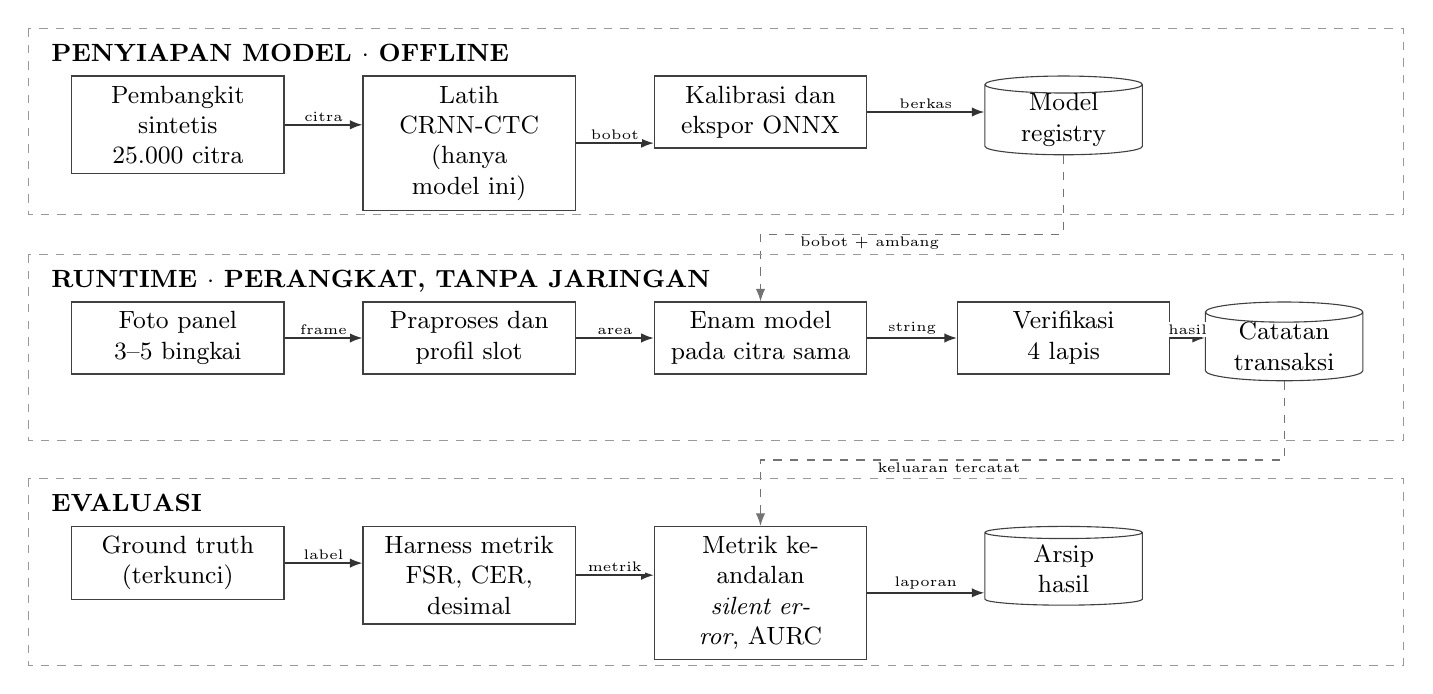
\begin{tikzpicture}[
  x=1cm, y=1cm,
  kotak/.style={rectangle, draw=black!75, fill=white, align=center,
                text width=2.45cm, inner sep=3.5pt, font=\small},
  simpan/.style={cylinder, draw=black!75, shape border rotate=90,
                 aspect=0.20, minimum height=1.00cm, minimum width=2.00cm,
                 align=center, font=\small, inner sep=0pt},
  panah/.style={-{Latex[length=1.6mm]}, draw=black!80, semithick},
  panahputus/.style={-{Latex[length=1.6mm]}, draw=black!55, dashed},
  lbl/.style={font=\tiny, inner sep=1pt, fill=white},
  judul/.style={font=\small\bfseries, anchor=north west}
]

% ===================== JALUR 1 =====================
\node[kotak, anchor=north] (gen)  at (2.05,0.72) {Pembangkit sintetis\\ 25.000 citra};
\node[kotak, anchor=north] (latih)at (5.75,0.72) {Latih CRNN-CTC\\ (hanya model ini)};
\node[kotak, anchor=north] (eksp) at (9.45,0.72) {Kalibrasi dan\\ ekspor ONNX};
\node[simpan, anchor=north] (reg) at (13.30,0.72) {Model\\ registry};

\draw[panah] (gen.east)   -- node[lbl, above] {citra}  (latih.west |- gen.east);
\draw[panah] (latih.east) -- node[lbl, above] {bobot}  (eksp.west |- latih.east);
\draw[panah] (eksp.east)  -- node[lbl, above] {berkas} (reg.west |- eksp.east);

% ===================== JALUR 2 =====================
\node[kotak, anchor=north] (foto)  at (2.05,-2.15) {Foto panel\\ 3--5 bingkai};
\node[kotak, anchor=north] (pra)   at (5.75,-2.15) {Praproses dan\\ profil slot};
\node[kotak, anchor=north] (model) at (9.45,-2.15) {Enam model\\ pada citra sama};
\node[kotak, anchor=north] (verif) at (13.30,-2.15) {Verifikasi\\ 4 lapis};
\node[simpan, anchor=north] (catat) at (16.10,-2.15) {Catatan\\ transaksi};

\draw[panah] (foto.east)  -- node[lbl, above] {frame} (pra.west |- foto.east);
\draw[panah] (pra.east)   -- node[lbl, above] {area}  (model.west |- pra.east);
\draw[panah] (model.east) -- node[lbl, above] {string} (verif.west |- model.east);
\draw[panah] (verif.east) -- node[lbl, above] {hasil} (catat.west |- verif.east);

% ===================== JALUR 3 =====================
\node[kotak, anchor=north] (gt)   at (2.05,-5.00) {Ground truth\\ (terkunci)};
\node[kotak, anchor=north] (harn) at (5.75,-5.00) {Harness metrik\\ FSR, CER, desimal};
\node[kotak, anchor=north] (metr) at (9.45,-5.00) {Metrik keandalan\\ \textit{silent error}, AURC};
\node[simpan, anchor=north] (arsip) at (13.30,-5.00) {Arsip\\ hasil};

\draw[panah] (gt.east)   -- node[lbl, above] {label}  (harn.west |- gt.east);
\draw[panah] (harn.east) -- node[lbl, above] {metrik} (metr.west |- harn.east);
\draw[panah] (metr.east) -- node[lbl, above] {laporan} (arsip.west |- metr.east);

% ===================== KETERGANTUNGAN =====================
\draw[panahputus] (reg.south) -- ++(0,-1.00) -| 
  node[lbl, below, pos=0.32] {bobot + ambang} (model.north);
\draw[panahputus] (catat.south) -- ++(0,-1.00) -|
  node[lbl, below, pos=0.32] {keluaran tercatat} (metr.north);

% ===================== KOTAK JALUR =====================
\begin{scope}
  \draw[dashed, draw=black!40] (0.15,1.32) rectangle (17.62,-1.05);
  \draw[dashed, draw=black!40] (0.15,-1.55) rectangle (17.62,-3.92);
  \draw[dashed, draw=black!40] (0.15,-4.40) rectangle (17.62,-6.77);
\end{scope}

\node[judul] at (0.32,1.24) {PENYIAPAN MODEL $\cdot$ OFFLINE};
\node[judul] at (0.32,-1.63) {RUNTIME $\cdot$ PERANGKAT, TANPA JARINGAN};
\node[judul] at (0.32,-4.48) {EVALUASI};

\end{tikzpicture}
\end{document}
